%%%%%%%%%%%%%%%%%%%%%%%%%%%%%%%%%%%%%%%%%%%%%%%%%%%%%%%%%%%%%%%%%%%%
%%  The file contains the LaTeX shell for BIRS workshop reports.
%%
%%  The reports are being compiled into one volume so you must stick
%%  to the following.
%%
%%  Do not change/add anything before \begin{document}.
%%
%%  There is a list of packages you can uncomment and use.  
%%
%%  The use of TeX/LaTeX macros is NOT permitted.  Reports with macros
%%  will not be accepted. 
%%
%%  Please let LaTeX handle the numbering of your sections, equations, 
%%  figures and tables.
%%
%%  Do not be too concerned about page breaks etc.  These may change
%%  when your document is put into the volume.  We will make sure the
%%  page breaks look okay.
%%
%%  Please use thebibliography environment to do your references.  Use
%%  the format shown in the examples below.
%%
%%  Please use the \includegraphics for including images.  If you
%%  wish, graphics can be sent separately with comments in the tex
%%  file to indicate where they should be included and how big they
%%  they should be.
%%
%%  You can find all of the reports for the BIRS workshops online
%%  under the Publications link.  Select "BIRS 2003 Proceedings" to
%%  view all the reports.  The Scientific Director recommends the
%%  following reports as 'good' examples: Chapters 2, 6, 7, 9, 14, 15
%%  and 22.
%%
%%  Last revised on 24 March 2006.
%%%%%%%%%%%%%%%%%%%%%%%%%%%%%%%%%%%%%%%%%%%%%%%%%%%%%%%%%%%%%%%%%%%%%
\documentclass[12pt]{article}

\setlength{\textwidth}{6.0in}
\setlength{\textheight}{9in}
\setlength{\oddsidemargin}{0.5in}
\setlength{\evensidemargin}{0in}
\setlength{\topmargin}{-0.25in}
\pagestyle{myheadings}

%%%%%%%%%%%%%%
%% CLEVEREF %%
%%%%%%%%%%%%%%
%% order matters: hyperref before cleverref, and biblatex last
\usepackage{hyperref}
%% cleveref package for convenient hyper-referencing/citing:
\usepackage[nameinlink,capitalize]{cleveref}
%% The default cref format includes a space before the number, e.g.,
%% "§ 3" rather than "§3", so when using § it looks better to
%% define the cref format explicitly:
%% https://tex.stackexchange.com/questions/247538/remove-space-in-the-default-cref-command
\crefformat{section}{\S#2#1#3}
%% A space is still included when multiple sections are referenced,
%% but I think removing the space for multiple section refs would look
%% worse.
\crefname{section}{\S}{\S\S}
\Crefname{section}{Section}{Sections}
\crefname{equation}{Equation}{Equations}
\Crefname{equation}{Equation}{Equations}
\crefname{figure}{Figure}{Figures}
\Crefname{figure}{Figure}{Figures}
\Crefname{appsec}{Appendix}{appendices}

%%%%%%%%%%%%%%%
%% CITATIONS %%
%%%%%%%%%%%%%%%
\usepackage[sort&compress,numbers]{natbib}
\bibliographystyle{unsrtnat}

%%%%%%%%%%%%
%% LAYOUT %%
%%%%%%%%%%%%
% \usepackage[skip=1.5em]{parskip}
\setlength{\parskip}{0.5em plus0.5em}
\usepackage{enumitem}
\setlist[itemize]{noitemsep}

%%%%%%%%%%%%
%% MACROS %%
%%%%%%%%%%%%
\usepackage{xspace}
% \newcommand{\macpan}{\texttt{macpan2}\xspace}
\newcommand{\macpan}{\texttt{macpan2}\xspace}
\newcommand{\macpanOrig}{\texttt{McMasterPandemic}\xspace}
\newcommand{\R}{\texttt{R}\xspace}
\newcommand{\eg}{\textit{e.g.},\xspace}
\newcommand{\ie}{\textit{i.e.},\xspace}

\usepackage{times}

%%  Please uncomment any package you need to use.
%% 
%%  If you need to use any additional packages please email BIRS
%%   Programme Coordinator, birs@birs.ca, first.
%% 
%%  \usepackage{epsfig}
%% 
%%  \usepackage{amssymb}
%% 
%%  \usepackage{amsmath}
%% 
%%  \usepackage{amsthm}
%% 
\usepackage{graphics}
\usepackage{graphicx}
%% 

\begin{document}

\title{The Canadian Network for Modelling Infectious Diseases:
  Progress and Next Steps\\\medskip BIRS Workshop 23w5151}
\author{David Earn (McMaster University),\\ Caroline Colijn (Simon Fraser University),\\ Irena Papst (Public Health Agency of Canada)}
\date{12--17 November 2023}
\maketitle
\vspace{1in}  % This space is so the page break is approximately the
              % same as in the volume.

\tableofcontents

\section{Background \& Motivation}


Infectious disease modelling that aims to contribute to public health
decision-making has a long history, going back to Daniel Bernoulli’s
work on smallpox control in the 18th century.  In the early 20th
century, Ronald Ross developed a mathematical model to help identify
effective malaria control strategies, and Kermack and McKendrick
developed the foundations of modern mathematical epidemiology.  While
theoretical work on disease modelling continued, attention from
decision-makers and politicians was scarce until the 2001 Foot and
Mouth Disease epidemic in the UK, and the SARS epidemic in 2003.  Over
the last 20 years, the perception of mathematical modelling as a
valuable tool in the public health policy process has become more and
more common, especially in the context of influenza pandemic
preparedness, which set the stage for immediate, serious engagement
with modellers when the SARS-CoV-2 pandemic exploded in early 2020.

From the start of the pandemic, many disease modellers around the
world found themselves in constant demand from public health agencies
and policy-makers.  Recognizing the importance of this development,
NSERC invested \$10M with the aim of creating networks of disease
modellers and public health professionals and policy-makers.  25\% of
the investment (\$2.5M) was allocated to our
\href{https://canmod.net/}{CANMOD network} (the remaining 75\% was
allocated to four other networks).

CANMOD aims to increase Canada’s capacity for data-driven emerging
infectious disease modelling (EIDM) to directly support short, medium,
and long-term public health decisions. Our network comprises
collaborative teams of modellers, statisticians, epidemiologists,
public health decision-makers, and those implementing and delivering
interventions. The questions we are tackling are grounded in public
health needs and generated in partnership between research
investigators and knowledge users -- public health leaders, health
administrators and policy-makers. This collaborative research supports
data collection, curation and access, with the hope that it will
increase the speed with which critical information is made available.
While the network initially focussed on addressing questions of
immediate relevance in the shorter term, we are continuing this
approach with longer-term challenges in mind, building a trajectory of
enhancing modelling expertise and capacity in infectious disease in
Canada. As researchers have moved from the daily challenges of
decision-making during the COVID-19 pandemic to working on longer-term
policy questions, CANMOD is building and coordinating national
capacity in infectious disease modelling at the forefront of public
health. This capacity will position public health across Canada for
better control of any infectious disease, and will build better
preparedness and resilience in case of future pandemics. While CANMOD
is primarily concerned with Canadian pandemic preparedness and
infectious disease control, the research resulting from the network’s
activities will provide an international benefit since emergent
pathogens pose a universal, global threat.

We are providing extensive experiential training opportunities for
postdoctoral fellows (PDFs), graduate and undergraduate students at
the intersection of infectious disease modelling, public health policy
and decision making. CANMOD is committed to increasing equity,
diversity, and inclusion in the next generation of infectious disease
modellers. Our trainees are well-placed for quantitatively-oriented
careers in academia, industry and the public sector, both in Canada
and abroad.

It is our experience that when modellers and statisticians undertake
research driven by public health and policy-relevant questions, it
leads to new science and methodology. If these questions were easy to
answer, public health researchers and institutions would answer them
with existing tools. However, even with established approaches to
infectious disease modelling, there remains a need to adapt and design
novel approaches and tools to address new and nuanced scientific
questions; to integrate noisy, incomplete, and abundant data streams;
and to capture fundamental properties defining local context. The
COVID-19 pandemic in Canada has made clear the urgent and immediate
need for modelling of local context to inform decisions that are often
implemented in local jurisdictions, and across diverse epidemiologic
and health system contexts. Effective public health benefits from the
support of engaged modellers who understand the local data, local
epidemiological, socio-cultural, and health-system contexts, and who
are passionate about collaborating on public health research
problems. Our 44 co-applicants and dozens of collaborators have been
engaged in this kind of work since the beginning of the COVID-19
pandemic, and are ideally placed to ensure that the collaborations we
continue to build are effective. The enthusiasm of public health
institutions is clear from the level of engagement to date, the
regular use of our research results in decision-making, and from
numerous and enthusiastic letters we have received from a wide range
of public health institutions across Canada, spanning municipal,
regional, provincial and national jurisdictions. Some of the
high-priority scientific questions that have emerged through this
collaborative research and were discussed at the workshop
are summarized below.

CANMOD’s multi-disciplinary and multi-sectoral network is addressing
all infectious disease challenges with principles of equality,
diversity and inclusion through its recruitment, training, and
research, and through events like the November 2023 BIRS meeting that
this report summarizes.


\section{Structure of the Workshop}

To be ripped from the proposal + the online schedule

\section{Presentation Highlights}

\subsection{Special Sessions}

\subsubsection{Historic Disease Data Portal}

To be drafted by Steve.
\subsubsection{Surveillance Discussion}
\label{sec:surv-disc}


The effective collection, analysis, and application of diverse infectious disease surveillance data streams are paramount to understanding and managing infectious disease threats. Recently, the WHO released guidelines for ethical public health surveillance, arguing that societies have an obligation to design and deliver effective public health surveillance. We explore infectious disease surveillance from the point of view of researchers, primarily infectious disease modellers, working at the interface between research and policy during the COVID-19 pandemic.

We held a roundtable discussion on surveillance.
Our discussion moved through infectious disease surveillance (and related) data types, their collection, and the ways in which they inform surveillance questions.


There is a wide range of data types that play important roles in understanding and managing infectious diseases; here we focus primarily on respiratory infectious disease and issues that arose during the COVID-19 pandemic. Many of these apply to influenza, RSV and other respiratory illnesses, and some (like the “First 100”) are relevant mainly to a potential new emerging infectious disease. 

Data streams include:
\begin{itemize}
\item \textbf{Lab-Based Data}: These data comprise the results of testing, which indicate whether an individual is infected, for a specific virus or infectious agent. There is typically some stratification by age, perhaps sex, location. 
\item \textbf{Case-Level Data}: This refers to detailed information on each case, such as line lists and contact tracing records.
\item \textbf{First 100 cases}: especially in the early stages of a new emerging infectious disease, this can provide essential characterization of the course of infection, exposure, pace of transmission, severity, clinical needs
\item \textbf{Genomics}: Genomic analysis (viral sequencing) helps track the mutation and spread of pathogens. Interpretation can be challenging, due to lack of linkage with epidemiological, clinical, demographic or immunity data, and due to sampling that is a mixture of travel-related cases, random sampling (but only within the schema of the testing system), and priority sequencing (for example of outbreaks)
\item \textbf{Outcomes}: hospitalization, acute care needs, by age (aggregate; individual outcomes would be in individual-level data) 
\item Tools like the \textbf{WHO Ordinal Scale}, which measure the severity of cases: however, there are challenges in standardizing these scales across different regions, hospitals, or countries, particularly when data is incomplete or inconsistent. If hospitals are overwhelmed, data on these scales will be impacted 
\item \textbf{Mortality Data}: this can lack timeliness, consistency across jurisdictions and completeness
\item \textbf{Immunity}: serology, vaccination levels
\item \textbf{Denominator/population-level data}
\end{itemize}


Additional non-health data that are relevant for interpretation and modelling of infectious disease surveillance data: 
\begin{itemize}
\item  \textbf{Policy data}:
\item \textbf{Behavioural data}: this is a large area, not typically considered part of routine respiratory surveillance data. It comprises mobile phone  (mobility) data, contact data derived from surveys, and other information about behaviour relevant to infectious disease transmission (use of NPIs, response to illness). This could also include information about test-seeking and health-care-seeking behaviour. 
\item \textbf{Travel and Movement Data}: Data on travel, both international and interprovincial
\item \textbf{Demographic changes over time}
\end{itemize}

Our discussion continued, to explore the epidemiological pyramid, which connects some of these layers of data together, conditional on others. For example, the relationship between detected cases and infections depends on test seeking, testing policy, immunity including vaccination, and the intrinsic severity of the virus variant, to name a few.

Several participants emphasized the importance of data linkage, and of context.  The integration of genomic data with epidemiological, clinical, vaccination, and demographic data is especially important. Without these connections, the full potential of genomic insights remains largely untapped. For instance, determining whether a new variant is transmitting among vaccinated individuals requires a synthesis of genomic, epidemiological and vaccination data. Determining severity requires information about clinical outcomes, in individuals with and without the new variant.

One of the main focal points for our discussion was to solicit modellers' input on how infectious disease surveillance data could be made more useful to modellers, as throughout the pandemic, modellers were asked to support policy-makers in questions about COVID-19 scenarios, forecasts and healthcare impacts.

The utility of data is intrinsically linked to the specific question it aims to answer. For prediction purposes, it’s useful to clarify what is being predicted. For example, predicting the dynamics of infections requires different data compared to predicting the impact on healthcare resources. The following aspects were identified as important ways that surveillance systems could take these needs into account.  

{\bf Timeliness}: The value of surveillance data is heavily dependent on its currency. Real-time or near-real-time data acquisition enables public health officials to respond swiftly to emerging threats, adjust strategies based on current trends, and predict future outbreaks with greater accuracy. Delayed data can lead to missed opportunities in containing and mitigating outbreaks.

{\bf Testing policy}: Knowing who is being tested and recognizing any shifts in this demographic is important. Changes in testing patterns can significantly impact the interpretation of surveillance data. For instance, if testing becomes more widespread or targeted at specific groups, this shift needs to be factored into the analysis to avoid misinterpretation of disease trends.

{\bf Stratification (lab data)}: Stratifying lab data by variables such as age, sex, and immune status can help unpack nuance and changes in testing, and help build a more nuanced understanding of a disease's impact and spread. Stratification may be helpful in understanding changes in testing policy or test-seeking behaviour. Including vaccination status (including the recency of vaccination and time since the last dose) adds another layer of depth, enabling improved understanding of immunity in the population and the effectiveness of vaccines against current strains.

{\bf Linkage}: Linking across datasets enhances the richness and depth of analysis and adds value. For instance, connecting laboratory data with clinical outcomes, vaccination records, and demographic information provides a comprehensive picture of the disease's impact, spread, and evolution (and see above for the benefits of genomic data with linkage).  

{\bf Consistency}: In addition to the above, it is important for data to be consistently reported across local jurisdictions, hospitals, and laboratories, and as such, the creation of standards can help move the needle forward when thinking about surveillance data for infectious disease modeling.



\subsubsection{\macpan Modelling Software}
\label{sec:macpan}

\textit{Steven C Walker, Irena Papst}

\macpanOrig is an \R package for compartmental modelling that was developed to provide forecasts and insights to public health agencies throughout the COVID-19 pandemic. Forecasts created with \macpanOrig were prepared for the Public Health Agency of Canada, the Ontario Science Table, the World Health Organization, and Public Health Ontario. Much was learned about developing general purpose compartmental modelling software during these experiences, but the pressure to deliver regular forecasts to these organizations made it difficult to focus on the software itself. With the support of CANMOD, the \macpan project was launched to re-imagine \macpanOrig, building it from the ground up to address lessons learned while responding to a global public health emergency.

The special session on \macpan started with a presentation by Steve Walker introducing the project. Steve traced the history of \macpanOrig and \macpan, using it to argue that impactful modelling requires many interdisciplinary steps along the path from epidemiological research teams to operational decision-makers. Researchers must quickly tailor a model to an emerging public-health concern, validate and calibrate it to data, work with decision-makers to define model outputs useful for stakeholders, configure models to generate those outputs, and package up those insights in an appropriate format for stakeholders. \macpan targets bottlenecks along this path that can be solved with thoughtful software engineering. The goal is to ease the software development burden on modellers, especially when they are working on an urgent public health response, so that they can devote their time and energy to the modelling itself.

After discussing the project's history and motivation, the presentation transitioned to \newline exploring \macpan's modular model building, a key feature meant to address a commonly-encountered bottleneck in modelling. New public health concerns often demand new modules to be added to existing models. For example, as vaccines against COVID-19 were deployed, models needed to be modified to include vaccination. Even beyond responding to a public health emergency, a common paradigm in modelling (and in writing code) is to start simply and add complexity incrementally, testing outputs at every step of the way. Experience shows that it can be surprisingly difficult to add new modules to a modelling pipeline if your existing toolkit is not designed for modular model building. Steve briefly reviewed existing approaches to modular compartmental modelling based on mathematical tools from graph theory and category theory. Steve described how modules in \macpan can be represented by tables (like tables in a database), and that widely-understood table manipulation tools (like join and group-by) can be used to combine modules without the need for advanced mathematical concepts.

After the presentation, participants were invited to a hands-on session to explore \newline \macpan, led by Steve Walker, Irena Papst, and Ben Bolker. There were roughly 20 participants in the session, representing a wide range of career phases, from graduate students to tenured faculty. We started the session by helping particpants download and install the software on their computers. There were several installation hiccups that we were able to troubleshoot on the fly. These issues gave us valueable insight into potential difficulties deploying this software more widely, which will be addressed in future versions of the software.

We then invited participants to work through a \href{https://github.com/canmod/macpan2/blob/4b9812d4b05f3e959f2f84f4712d72a681b06e6c/vignettes/quickstart.Rmd}{getting started vignette} to enable them to further familiarise themselves with the software's model specification grammar, which enables modular model building. The vignette walks users through specifying a very simple epidemiological model, and then introduces software features that make it easy to add additional structure to models, such as modules for multiple infection types (\eg asymptomatic, symptomatic), multiple locations (often referred to as ``metapopulation'' models), stratification by vaccination status, and more. The vignette specifically works through the example of specifying a two-strain model while demonstrating \macpan functions key to easily specifying ``structured'' models.

After participants worked through the vignette, some worked on specifying other models in \macpan, as a way to test their understanding of the model specification grammar and to experiment with other features of the package. Two participants worked together to try to specify a Lotka-Volterra predator-prey model, and their attempts revealed interesting points of friction in the software that have directly inspired further development. These attempts also inspired the addition of Lotka-Volterra models to \macpan's model library. Three participants independently provided the same feedback about how calibrating models to data is a bigger bottleneck than modular model building, which has inspired us to make existing calibration tools more accessible via the \macpan interface.

This session was the first \macpan training ever run, and overall, we received a lot of valuable feedback from participants on it. We continue to use this feedback to both improve guides for the software, as well as the software itself.

\subsection{Short Talks}
\label{sec:short-talks}

\subsubsection*{The CANMOD/EIDM Knowledge Graph}
\textit{David Price, DebateGraph}

The opening talk explored the content, structure, rationale of the EIDM dynamic knowledge graph (\url{https://eidm-mmie.net}), which is being developed by CANMOD to support, document, and interconnect the work conducted across the five EIDM networks. Workshop participants were guided through the exploration and use of the graph as a repository of knowledge and as a resource for search-based discovery. As illustrated in the figures below, the graph identifies and interweaves multiple aspects of the EIDM initiative, including: the participants, their organizational affiliations and collaborations, research interests, publications, goals, datasets, software, and training materials. Interactive visualisations make it simple to traverse the graph, focusing on the immediate connections around the individual elements and zooming out to see the wider patterns and connections emerging as the network continues to grow.

\begin{center}
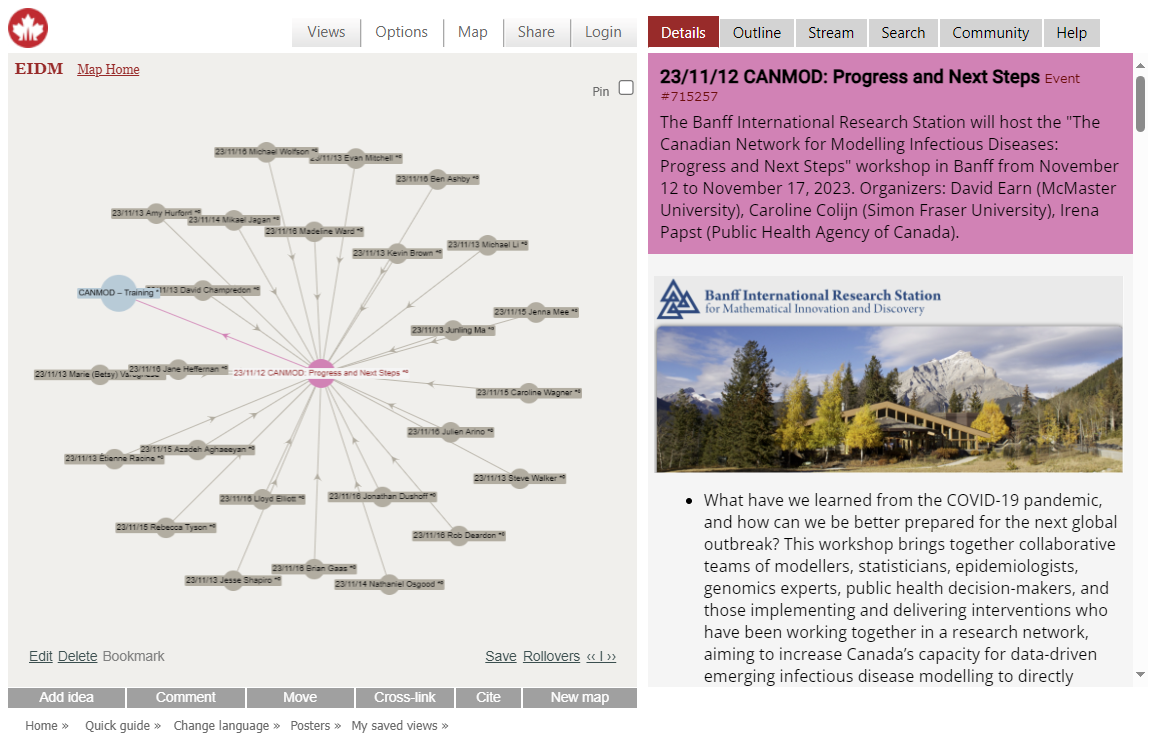
\includegraphics[width=\textwidth]{talk_summaries/EIDM_CANMOD.png}
\end{center}

Efficient coverage for newly developed vaccines requires knowing which
groups of individuals will accept the vaccine immediately and which will
take longer to accept or never accept.

In this study, we assumed that, within the context of COVID-19
vaccination, non-vaccine refuser Americans behaved as either
success-based learners, making decisions based on
others\textquotesingle{} satisfaction, or as myopic rationalists,
attending to their own immediate perceived benefit.

We used COVID-19 vaccination data to fit a mechanistic model capturing
the distinct effects of the two types on the vaccination progress.

We estimated that about half of Americans behaved as myopic rationalists
with a high variation across the states.

The proportion was correlated with the vaccination coverage, proportion
of votes in favor of Democrats in 2020 presidential election, and
education score.

The findings reveal the impact of the proportions of the decision-makers
on the vaccination speed and, consequently, overall vaccination
coverage.

Azadeh Aghaeeyan

Brock University

\subsubsection*{Antigenic evolution of SARS-CoV-2 in immunocompromised hosts}
\textit{Ben Ashby, Simon Fraser University}

Prolonged infections of immunocompromised individuals have been proposed as a
crucial source of new variants of SARS-CoV-2 during the COVID-19 pandemic.
Longitudinal sampling of SARS-CoV-2 from immunocompromised hosts reveals
evidence of accelerated adaptation relative to the wider population. In
principle, sustained within-host antigenic evolution in immunocompromised hosts
could allow novel immune escape variants to emerge more rapidly, but little is
known about how and when immunocompromised hosts play a critical role in
pathogen evolution. I will discuss how a relatively simple mathematical model
can provide powerful insights into the effects of immunocompromised hosts on the
emergence of immune escape variants. Specifically, when the pathogen does not
have to cross a fitness valley for immune escape to occur, a small number of
immunocompromised hosts have no qualitative effect on antigenic evolution at the
population-level. But if a fitness valley exists, then persistent infections of
immunocompromised individuals allow mutations to accumulate so that the fitness
valley can be traversed, thereby facilitating large jumps in antigenic space at
the population-level. Our results suggest that better genomic surveillance of
infected immunocompromised individuals and better global health equality,
including improving access to vaccines and treatments for individuals who are
immunocompromised (especially in lower- and middle-income countries), may help
to prevent the emergence of future immune escape variants of SARS-CoV-2.


\subsubsection*{Better modeling through chemistry: quantifying COVID vaccine hesitancy}
\textit{Brian Gaas, Government of Yukon}

Much of the literature on vaccine hesitancy focuses on whether an individual receives a vaccine. However, the rate of vaccination---the number of people getting vaccinated in a given amount of time---is equally important. This work presents a conceptual framework for understanding and predicting vaccine adoption rates, following the transition state theory of chemistry. 

The vaccine uptake framework hypothesizes people will only get vaccinated if their personal Vaccine Motivation exceeds a population-averaged Vaccine Hesitancy. Within the framework, Vaccine Motivation and Vaccine Hesitancy are functionally equivalent to temperature and activation energy, respectively, within the Arrhenius equation. The proportion of unvaccinated individuals getting vaccinated per unit time is related to the negative exponential of the Vaccine Hesitancy Ratio, defined as Vaccine Motiviation divided by Vaccine Hesitancy. Neither Vaccine Motivation nor Vaccine Hesitancy are observable, but the Vaccine Hesitancy Ratio for a given time period can be estimated as the negative log-odds of vaccination status (individuals who changed vaccination status versus individuals who did not change status within that period). Logistic regression can be used to test whether the Vaccine Hesitancy Ratio varies over time, since it has the same log-odds form. 

Dose 1 uptake rates from the Yukon (Canada) for COVID-19 were analyzed using the vaccine uptake framework. The population could be clustered into four groups of people based on how the Vaccine Hesitancy Ratio changed over time: low, medium, and high Vaccine Hesitancy Ratios, and one group who never got vaccinated. Further work could include applying clustering algorithms to better differentiate groups, identifying predictors that classify individuals into each of the four groups, and applying the vaccine uptake framework to forecast future dose uptake or uptake rates of different vaccines.
\subsubsection*{Multi-Pathogen Agent-Based Models for Disease
Surveillance and Mitigation}
\textit{Caroline Wagner, McGill University}

Understanding the dynamics of emerging infections and
the efficacy of detection technologies in the context of the endemic
circulation of other pathogens is a critical aspect of effective public
health responses against infectious diseases. The use of compartmental
models to simulate the effectiveness of different detection technologies
is complicated by the importance of heterogeneity in numerous aspects of
these systems, including underlying patterns of technology distribution
within a population and variable in-host immune responses. Compartmental
models also present challenges when modeling large numbers of
co-circulating pathogens with specific disease characteristics and
immunological rules for pathogen-pathogen interactions. In light of
this, we present Pathosim, a multi-pathogen agent-based model (ABM) that
builds on the open-source COVID-19 model Covasim. Like Covasim, Pathosim
allows for flexible population and transmission network structures, and
can simulate individual in-host viral kinetics, the implementation of
pharmaceutical interventions, and testing and quarantine procedures. In
addition, Pathosim allows for the flexible characterization of any
pathogen of interest along with the specification of immunological rules
for pathogen-pathogen interactions (i.e. cross-immunity and altered
disease course during co-infection). We then demonstrate the utility of
Pathosim in terms of simulating and modeling various detection and
surveillance systems including protocols for serosurveillance and
early-detection systems based on sequencing data.


\textbf{Presenter}: David Champredon

\textbf{Title}: Academic collaborations to improve wastewater-based modelling at the Pubic Health Agency of Canada

\textbf{Abstract}

Since the COVID-19 pandemic, the surveillance of respiratory viruses in municipal wastewater has emerged as a valuable new data source for modellers.
However, there are still many unknowns regarding the various causes that can impact the viral concentration in wastewater during the journey of viruses in the sewer system.
Understanding the processes that can affect viral concentration in wastewater is critical for epidemiological surveillance at the Public Health Agency of Canada, and it involves many scientific fields, not all represented within the Agency.
In this talk, I highlight several projects done in collaboration with academic groups that brought their expertise to help better understand how various processes can impact viral concentration in wastewater. I also present the different ways academic groups can collaborate with PHAC.






























\section{Evan Mitchell - Talk Summary}

How many infections, hospitalizations, and deaths did COVID-19 vaccines prevent during the pandemic in Canada? This talk presents research aimed at answering this question. A compartmental model was fit to daily infection report and hospitalization occupancy data for Ontario from the start of the pandemic through the end of the Delta wave in December 2021. We use this model to simulate counterfactual scenarios where vaccines were not present, vaccine introduction was delayed 60 days, or vaccines were 25\% less effective. Results from these simulations show that the predicted numbers of infections, hospitalizations, and deaths would be orders of magnitude larger than they actually were. To follow this up, we consider the effects of introducing a hypothetical stay-at-home order in an attempt to control these counterfactual scenarios. Our main finding from these explorations is that we would have a much easier time controlling the situation in the case of less effective vaccines than in the other two cases, suggesting that it is important to release a vaccine as early as possible during a pandemic even if that vaccine is less effective than it might be otherwise. We are currently in the process of extending these results to five other provinces: Alberta, British Columbia, Manitoba, Qu\'{e}bec, and Saskatchewan.



Title: Modelling Immunity

Jane Heffernan

Abstract: ‘Immunity’ is both a population- and an individual-level characteristic. We have developed individual- and population-level models of immunity using in-host modelling of vaccination, immune system and infection dynamics, and epidemiological models of disease spread and public health programming. In this talk, we will discuss the multi-level models of immunity and discuss their integration, which can be used to inform public health decision-makers. We will focus on COVID-19 in Ontario.


\subsubsection*{Conceptual models of immunity}
\textit{Jonathan Dushoff, McMaster University}

A better understanding of patterns and processes underlying
cross-immunity is needed to better understand future dynamics and
burden of important diseases. Simple dynamical models of
cross-immunity can often be classified as either history-based
(classifying individuals by history of infections), or status-based
(classifying individuals by what strains they are currently
effectively immune to). There is a very strong analogy between these
classifications and those of “leaky” and “polarized” vaccine models.

This talk discussed the importance of immune-boosting---that is,
enhanced immune protection following an unsuccessful infection
challenge---and demonstrated that a model with boosting provides a
practical way to bridge between the dynamics of these two paradigms,
while arguing that this mechanism is highly biologically relevant.
Differences in such conceptual assumptions can lead both to different
estimates of vaccine effectiveness, and different predictions about
future dynamics.


{\bfseries
Association between Delayed Nursing Home Outbreak Identification and
SARS-CoV-2 Infection and Mortality in Ontario, Canada

Kevin Brown
}

Delayed outbreak identification is likely an important driver of respiratory
infection transmission in nursing homes. Most studies examining outbreak
identification have been descriptive and there are no measures of delayed
outbreak identification in nursing homes. We conducted a longitudinal cohort
study of SARS-CoV-2 outbreaks from 623 nursing homes in Ontario, Canada in the
March 1, 2020 to November 14, 2020 period prior to the rollout of COVID-19
vaccination. Our exposure was the timeliness of outbreak identification, defined
as late ($\ge3$ resident-days of infection pressure) versus early
($\le2$ resident-days of infection pressure) on the date of outbreak
identification. Residents were considered to contribute infection pressure from
2 days prior to onset to 8 days afterwards while non-residents (including staff
and visitors) were not considered to contribute infection pressure. Our outcomes
were 30-day secondary infections and mortality, defined as the proportion of at
risk residents with a laboratory-confirmed SARS-CoV-2 infection with onset
within 30-days of the outbreak identification date, and mortality among these
residents. We identified 632 SARS-CoV-2 outbreaks across 623 Ontario nursing
homes during the study period. Of these, 230 (34.3\%) outbreaks were identified
late. Outbreaks identified late had higher secondary
infections (10.3\%, 4,437/43,078) and mortality (3.2\%, 1374/43,078) compared to
outbreaks identified early (infections: 2,015/61,061, $p<0.001$, mortality: 0.9\%,
579/61,061, $p<0.001$). After adjustment for 12 nursing home risk factors, the
incidence of secondary infections in outbreaks identified late was 2.90-fold
larger than that of outbreaks identified early (OR$=$2.90, 95\%CI: 2.04, 4.13).
Each 1-person-day increase in infection pressure at the time of outbreak
identification was associated with an 1.10-fold increase in the secondary
infections (OR$=$1.10, 95\%CI: 1.08, 1.12) and a 1.07-fold increase in secondary
mortality (adjusted OR$=$1.07, 95\%CI: 1.06, 1.09). In the nursing home setting,
SARS-CoV-2 outbreaks identified late evolved to be much larger than outbreaks
identified early. The timeliness of outbreak identification can be used to
predict the trajectory of an outbreak and plan for increased staffing demands,
infection control measures, and antiviral administration, with the goal of
mitigating harms to residents.

\subsubsection*{Assessing the Impact of Non-Pharmaceutical Interventions on COVID Prevalence Using A Predator-Prey Lotka-Volterra Model Approach}
\textit{Lisa Kanary, Public Health Agency of Canada}

Understanding the dynamics of disease transmission and effective
interventions is crucial due to a virus' rapid
spread. Non-Pharmaceutical Interventions (NPIs) play a vital role in
mitigating the spread of a virus through a population, especially when
pharmaceutical interventions are limited or ineffective.  Implementing
NPIs such as social distancing, face masks, hand hygiene, travel
restrictions, and quarantine measures has been essential in
controlling the pandemic and reducing the burden on healthcare
systems.

This study aims to investigate the relationship between NPIs and COVID
prevalence. By incorporating NPIs into a modeling framework, this
assessment will help determine the effectiveness of NPIs in reducing
the transmission and overall prevalence of COVID-19, and effectively,
disease in general.

To investigate the relationship between COVID prevalence and NPIs, we
employ a predator-prey Lotka-Volterra model. The predator-prey model
offers a theoretical framework that allows for the examination of the
impact of NPIs on COVID transmission dynamics and provides insights
into the effectiveness of these interventions in controlling disease
prevalence. The insights provided by these mathematical models can
inform decision-making processes for policymakers, public health
officials, and researchers, and can guide the development of targeted
interventions, helping to control the spread of the virus and mitigate
its impact on public health and society. Several methods for fitting
model coefficients will be explored in this exercise.


\section{Toward Support for Epidemic Preparedness via Digital Twin Data
+ ``Think Big''
Proposal}\label{toward-support-for-epidemic-preparedness-via-digital-twin-data-think-big-proposal}

Michael Wolfson, uOttawa, Banff Centre, November 16, 2023

Abstract / Summary

An essential component for pandemic preparedness is adequate data
supporting ongoing analytical capacity. Since support for specialized
pandemic-oriented data collection (+ analytical capacity) tends to wane
between acute events, data for pandemic preparedness should, as much as
possible, be designed to be useful during quiescent periods. One such
kind of data is a realistic but synthetic ``digital twin'' that closely
resembles detailed census data but is non-identifiable, hence
non-confidential. Such digital twin data would provide individual-level
details of Canada's population by small area geography and a range of
socio-economic and infectious disease-relevant characteristics,
substantially reflecting real-world heterogeneities. In turn, these data
could provide a richly textured basis for more sophisticated infectious
disease modeling, especially with regard to contact patterns more
readily incorporated into agent-based modeling as compared to the more
usual compartment models.

Such a digital twin database could be constructed by starting first with
published census cross-tabs at the census tract level using simulated
annealing, and then synthetically matching (with replacement) individual
and household level records from census public use files, thereby
substantially preserving important kinds of correlations. In addition,
data from other key microdata files like the Canadian Community Health
Survey (CCHS), the Labour Force Survey (LFS), and the time use results
from the General Social Survey could also be synthetically matched. As
these data sources are either already in the public domain, or versions
could be so constructed, the resulting digital twin would also be
non-confidential, hence completely open data.

Constructing this digital twin database and regularly updating it would
incur considerable costs. However, it would also have a much broader
range of uses than only to support epidemic modeling. With a broad range
of users, it would be more easily sustained over time as a new and
important addition to Canada's statistical system.

In order to keep the digital twin data current, ``nowcasting'' using a
public domain version of Statistics Canada's DEMOSIM model could be
used, along with other regular monthly data sets including the LFS and
CCHS.

With the advent of an epidemic and the imposition of public health
measures such as lock downs, behaviors would change. These could be
tracked via appropriately anonymized yet still geographically detailed
real-time cell phone mobility data.

In sum, a well-conceived digital twin database could provide both a
substantially improved real-time basis for infectious disease modeling
and a substantial addition to Canada's statistical system that would
have a broad range of other uses, thereby assuring its longer terms
sustainability.

Based on some of the preceding discussion in the conference, this
presentation also offered the suggestion of ``thinking big'' --
developing a brief for senior officials and governments outlining the
idea of a digital twin along with other key improvements in linkable and
coherent data flows such as infections, hospitalizations, vaccinations,
and genotyping of infections. While this kind of initiative is not
something fundable using the current Canadian and provincial granting
council structures, there is a window of opportunity with recent reports
on data from the Public Health Agency of Canada and Health Infoway, and
the 2023 federal budget proposing over half a billion dollars for health
data. There is also the recent Report of the Advisory Panel on the
Federal Research Support System which could well open up the right kind
of funding opportunities.


\subsubsection*{Within-host diversity of SARS-CoV-2 across animal host
species}
\textit{Jesse Shapiro, McGill University}

Viral transmission across different host species makes eradication very challenging and also opens new evolutionary trajectories for the virus. Since the beginning of the ongoing COVID-19 pandemic, SARS-CoV-2 has been transmitted from humans to several different animal species, and novel variants of concern could plausibly evolve in a non-human animal. Previously, using available whole genome consensus sequences of SARS-CoV-2 from four commonly sampled animals (mink, deer, cat, and dog) we inferred similar numbers of transmission events from humans to each animal species but a relatively high number of transmission events from mink back to humans (Naderi et al., 2023). In a genome-wide association study (GWAS), we identified 26 single-nucleotide variants (SNVs) that tend to occur in deer, more than for any other animal, suggesting a high rate of viral adaptation to deer. Here we show that deer harbor more intra-host SNVs (iSNVs) than other animals, providing a larger pool of genetic diversity for natural selection to act upon. Deer contain more distinct viral lineages than other animals, indicating possible co-infections, but this effect is unlikely to explain the overall higher diversity within deer. Compared to other animals, iSNV frequencies in deer are skewed toward higher frequencies, which is unexpected after a recent population bottleneck or population expansion and therefore suggests that deer are sampled relatively late in the course of infection. Combined with extensive deer-to-deer transmission, the high levels of within-deer viral diversity help explain the apparent rapid adaptation of SARS-CoV-2 to deer.

Hi All,

Thanks for sharing the report. I am not sure if it is possible to include the summary of the DUT presentation:

The Decision Uncertainty Toolkit
Megan Wiggens, Marie Betsy Varughese, Ellen Rafferty, Jeff Round, Sasha van Katwyk, Erin Kirwin

Presented by: Marie Betsy Varughese, Institute of Health Economics

Infectious disease (ID) models played an important role in decision making during the COVID-19 pandemic. While ID modelling has methods to
address structural and parameter uncertainty, communicating decision uncertainty is another important interface between ID modelers and
decision-makers. This talk presented the Decision Uncertainty Toolkit aimed to address and develop methods for communicating uncertainty to
decision makers where there are multiple policy options. The toolkit includes visualizations, risk measures, descriptions, and interpretations.
As this work is on-going, we included an opportunity for further involvement through a planned workshop in 2024 to try out the tool and provide
additional feedback on the codes, visualizations, and descriptions.

Thanks,
Betsy
\subsubsection*{The need to evaluate existing data resources and knowledge gaps to support future needs for respiratory disease surveillance and modelling}
\textit{Michael Li, Public Health Agency of Canada}

Infectious disease surveillance and health data sharing have always
been topics of discussion, even before the SARS-CoV-2 pandemic. The
SARS-CoV-2 pandemic amplified the value of these discussions,
providing researchers and government scientists with a small glimpse
of the data possibilities—such as the high frequency of time series
data reporting positive cases, testing, sequencing, hospitalization,
and death. However, what we had for SARS-CoV-2 is still far from the
ideal data structure (e.g., linkable data, health status, etc.) needed
to learn more about the questions of interest. Before we can make
further progress, the capacity diminishes due to low-frequency/quality
reporting.

Lack of surveillance and data sharing are often viewed as the same
problem; however, it is important to recognize that they are separate
issues.  Our focus should be on learning from data, not just on the
data itself. The key is not sharing data per se, but fostering
effective collaborations to obtain information from data—referred to
as ``data-info or data-knowledge sharing''

This talk proposes a pandemic and peacetime preparedness vision
called the ``PREP'' vision, which stands for Profiling, Reflection,
Exploring alternative options, and Proof of concept. Profiling
identifies what different people want to know and the bottlenecks of
knowledge gaps.  Reflection evaluates existing resources used to seek
answers to understand what needs improvement. Exploring alternative
options goes beyond the current status quo to see what can be done to
improve access and, eventually, enhance the resources. Lastly, a proof
of concept aims to validate whether the ideas are worth implementing
using the model world.

\section{Testimonials}

\begin{quote}
{\it ``The CANMOD BIRS workshop was a fabulous experience, both overall and in its specifics. Direct shuttles between Calgary and Banff, lodging and included meals at the site of the conference, on-hand IT staff for presentations, giant mountains to look at... I'm not sure what else one might want for logistics. I imagine conference attendees everywhere were happy to see the people behind the Zoom and Teams screens for the first time in a few years, and this was no exception. It is perhaps the goal of every conference to provide a venue where people can learn what their colleagues are up to, and collaborate on future projects. The CANMOD workshop succeed admirably in this, and I am currently following up with a few different groups on work that was presented. My two complaints are me not bringing climbing shoes, and eating too much at the buffet dinners... both which are perfectly good problems to have.''}

\hfill Brian Gaas, Government of Yukon
\end{quote}
\begin{quote}
\textit{``The CANMOD BIRS workshop was easily one of the best I have ever attended. All of the talks were excellent and the focus of the workshop on infectious disease modelling meant all of them were of interest to everyone. Communal meal times were also a great way to get to interact with other attendees and the small workshop size meant that, by the end of the four days, I was able to have a conversation with everyone at least once. I thoroughly enjoyed my time in Banff and left the workshop feeling reinvigorated about working on infectious disease research projects.''}

\hfill Evan Mitchell, McMaster University
\end{quote}
\begin{quote}
{\it ``As a infectious disease epidemiologist working as a scientist at Public Health Ontario, I know the acute need for strong connections between the academic mathematical modeling community, public health, and government decision makers. At the BIRS-CANMOD meeting in November 2023, I made great connections that will support future public health responses to infectious disease threats, by supporting such connections. In addition to excellent applied presentations, we had beneficial discussions about how to strengthen public health surveillance data for respiratory infections, that could help support more robust forecasting of respiratory infections in the future.''}

\hfill Kevin Brown, Public Health Ontario
\end{quote}
\begin{quote}
{\it ``Attending the conference was an invaluable experience that provided me with a unique platform for fostering meaningful research connections and collaboration.  The opportunity to meet people in person was instrumental in developing new innovative ideas and projects geared towards enhancing future pandemic preparedness. The insights gained not only deepened my understanding of the research our CANMOD team is engaged in but also fueled a collective passion for addressing critical challenges.

This conference served as a catalyst for interdisciplinary discussions, sparking the exchange of ideas that have the potential to shape the future of pandemic response strategies. The immersive environment facilitated networking, enabling me to connect with professionals who share a commitment to advancing our shared goals and learn from the diverse expertise of others. The experience has underscored the importance of such gatherings, emphasizing the need for more opportunities like this in the future.''}

\hfill Lisa Kanary, Public Health Agency of Canada
\end{quote}

\section{Conclusion}

\begin{itemize}
    \item general conclusion: enthusiasm for continuing to collaborate and grow the EIDM networks in Canada
    \item mention and cite the charting the future paper
    \item will feed into the next iteration of a macpan2 workshop
\end{itemize}

A common experience since the start of the COVID-19 pandemic has been
that we often meet people first virtually, and potentially never
in-person.  A large proportion of CANMOD's co-applicants had never met
in-person before the BIRS workshop, and the opportunity to do so---for
those of us who were able to attend in Banff---was greatly
appreciated.  For both in-person and virtual participants, the
presentations and discussions were extremely valuable, and the
connections made during the meeting will influence research and public
health policymaking in the coming years.  These types of
events---which generate enthusiasm among participants for continued
interactions between academics, govenment scientists, and
policymakers---are critical to the vision for EIDM modelling in Canada
described in a white paper \cite{Lewi+23} drafted by several of the
attendees together with members of other EIDM networks at an earlier
BIRS meeting in January 2023.  We are certain that all the attendees
at the CANMOD BIRS workshop in November 2023 are looking forward to
continuing to contribute to the realization of that vision!



\bibliography{birs.bib}

%%\begin{thebibliography}{}

%%%  Sample references.  Please use this format.

%\bibitem{label1} C. Radin and M. Wolff, Space tilings and local isomorphism,
%\emph{Geometriae Dedicata} \textbf{42} (1992), 355--360.

%\bibitem{label2} B. Solomyak, Spectrum of dynamical systems arising
%from Delone sets. In \emph{Quasicrystals and Discrete Geometry,
%(J. Patera, ed.)}, Fields Institute Monographs, \textbf{10}, 265--275,
%American Mathematical Society, 1998.

%\bibitem{label3} P. Walters, \emph{An introduction to ergodic theory},
%Springer Graduates Texts in Mathematics, Springer-Verlag, New York, 1982.

%%\end{thebibliography}

\end{document}

